\section{Patchplots Library}
{
\tikzset{external/figure name/.add={}{patchplot_}}%
\label{sec:lib:patchplots}
\begin{pgfplotslibrary}{patchplots}
	A library for advanced |patch| plots. Its strength is the creation of patches with smooth boundaries and smoothly shaded colors.
	
	A |patch| plot is a plot in which each individual patch is available. Here, ``available'' means that the user provided each individual patch manually. This can be achieved by means of a long series of patches which have been concatenated in a suitable way (compare the description of |patch| plots in section~\ref{sec:pgfplots:3d:patch}) or by means of a mathematical expression which is sampled (compare the key |patch type sampling|). Most |patch type|s expect a series of point evaluations in a specific sequence.
	
	Note that even though each individual patch might have a smooth boundary, the |patchplots| library \emph{does not interpolate smoothly between adjacent patches}. Consequently, it is task of the one who creates the patches (which means: evaluated some function at its vertices) to ensure that patches can be glued together in an adequate way. This allows a lot of freedom, including both jumps and smoothly concatenated edges. 

	The |patchplots| library comes with a couple of inherently two--dimensional |patch type|s (including second order triangles/rectangular patches and cubic tensor product patches known for finite elements). Typically, these patches live in a three--dimensional axis. Often, they are used to visualize the surface of function values $f(x,y)$. The |patchplots| library ensures that such patches are drawn in a way which respects the current view. In particular, if a patch folds over itsself (which is possible), it is drawn such that foreground areas are in the foreground and background areas are in the background.

	The |patchplots| library comes with smoothly shaded patches. More precisely, both the boundary of patches and their color shading are smooth. Note, however, that the patch boundary typically has much more smoothness than the color shading. 

	The |patchplots| library also allows automatic conversion from a higher--order patch to triangles (triangulation) by means of the key |patch to triangles|. Furthermore, it features automatic |patch refines|.

	Use the |patchplots| library if you want to have smooth boundaries for your patches, or if you need advanced shadings, or if you want polygon plots, or if you want more freedom in one--dimensional patches. 

\subsection{Additional Patch Types}
\message{Underfull hbox is OK.^^J}%
\begin{pgfplotskey}{patch type=\mchoice{default,rectangle,triangle,line,quadratic spline,cubic spline,\\bilinear,triangle quadr,biquadratic,bicubic,polygon,coons,tensor bezier} (initially default)}
	The |patchplots| library supports several new |patch type|s in addition to the initially available choices (which are |rectangle|,|triangle| and |line|). The documentation of the two--dimensional choices from page~\pageref{key:patch:type} is repeated here.

	The new |patch type|s are discussed in detail on the following pages.
\end{pgfplotskey} % end the environment to simplify sectioning.

\subsubsection{One--Dimensional Patch Types}
	There are two new one--dimensional patch types, namely |quadratic spline| and |cubic spline|. Here, |patch type=|\declareandlabel{quadratic spline} consists of quadratic patches of $n=3$ vertices each. The vertices are interpolated exactly:
\begin{codeexample}[]
\begin{tikzpicture}
\begin{axis}[nodes near coords={(\coordindex)},
	title={\texttt{patch type=quadratic spline}}]
\addplot[
	mark=*,
	patch,
	patch type=quadratic spline]
coordinates {
	% left, right, middle-> first segment
	(0,0) (1,1) (0.5,0.5^2)
	% left, right, middle-> second segment
	(1.2,1) (2.2,1) (1.7,2)
};
\end{axis}
\end{tikzpicture}
\end{codeexample}
	\noindent In our example, the first segment interpolates $f(x)=x^2$ at the points $\{0,\nicefrac12,1\}$. The |quadratic spline| is actually nothing but piecewise Lagrangian interpolation with quadratic polynomials: it expects three points in the sequence `(left end), (right end), (middle)' and interpolates these three points with a quadratic polynomial. Unlike the default 1d |mesh| visualization (which uses |patch type=line| implicitly), you have to use the special syntax above (or the equivalent approach by means of |patch table|). Note that |patch type=quadratic spline| results in correct shapes, but uses \emph{just constant color} for each segment; high--order color shading is only supported approximately using |patch refines|.

	The |patch type=|\declareandlabel{cubic spline} is very similar: it expects patches of $n=4$ vertices and interpolates them with a cubic polynomial:
\begin{codeexample}[]
\begin{tikzpicture}
\begin{axis}[nodes near coords={(\coordindex)},
	title={\texttt{patch type=cubic spline}}]
\addplot[
	mark=*,
	patch,
	patch type=cubic spline]
coordinates {
	% left, right, left middle, right middle
	(-1,-1) 
	(1,1)  
	(-1/3,{(-1/3)^3})
	(1/3,{(1/3)^3})
};
\end{axis}
\end{tikzpicture}
\end{codeexample}
	\noindent Here, we interpolated $f(x)=x^3$ at the four equidistant points $\{-1,-\nicefrac13,\nicefrac13,1\}$ with a cubic polynomial (which is $x^3$). The |cubic spline| expects a sequence of patches, each with four coordinates, given in the sequence `(left end), (right end), (interpolation point at $\nicefrac13$), (interpolation point at $\nicefrac23$)'. It has limitations and features like |quadratic spline|, see above.

\subsubsection{Providing Patches by means of Mathematical Expressions}
	Most |patch type|s expect a specific number of vertices in a specific sequence. This is part of what the |patchplots| library is. But is is still tedious to provide this sort of data.

	For simple |patch type|s like |line,rectangle| and |bilinear|, you can provide the input coordinates with any of the input methods which are available for all other plot handlers. In particular, |line| is just a |sharp plot| (with individually colored segments) and |rectangle| is nothing but a |surf| plot. Note that both |rectangle| and |bilinear| also accept the standard matrix input (with scanlines, see |mesh/ordering| and its documentation). In summary: \emph{simple patch types accept a simple input format}.

\begin{pgfplotskey}{patch type sampling=\mchoice{true,false} (initially false)}
	There are some complicated |patch type|s. In particular, all |patch type|s of higher order (i.e.\ \verbpdfref{quadratic spline}, \verbpdfref{cubic spline}, \verbpdfref{triangle quadr}, |biquadratic|, |bicubic|) need more points than just their corners. For such patch types, you need to resort to |mesh input=patches|. That means you need to provide extra vertices and their function evaluation values in a specific sequence.

	The |patch type sampling| method allows to simplify the procedure for such complicated |patch type|s\footnote{Note that \texttt{patch type sampling} is more or less useless for simple patch types.}: it works together with |\addplot expression| and evaluates the mathematical expression at each of the required vertices (in the correct sequence):
\begin{codeexample}[]
\begin{tikzpicture}
  \begin{axis}
  \addplot[
	samples=5,domain=-3:3,
  	mesh,patch type=cubic spline,
  	patch type sampling,
	% avoid individual colors per segment:
  	blue,point meta=none,
  ]
  	{exp(-x^2)};

  % a second plot which shows the 
  % generated x positions:
  \addplot[
    mark=*,only marks,scatter,
	samples=5,domain=-3:3,
  	patch type=cubic spline,
  	patch type sampling,
  	point meta={exp(-x^2)},
  ]
  	{-0.1};

  % a third plot which shows the marks
  % without patch type sampling:
  \addplot[
    mark=*,only marks,scatter,
	samples=5,domain=-3:3,
  	point meta={exp(-x^2)},
  ]
  	{-0.15};

  \end{axis}
\end{tikzpicture}
\end{codeexample}
	\noindent The first plot above is almost a normal plot by expression. The |samples| and |domain| key controls the sampling procedure, and |blue,point meta=none| defines the global color to use. Note that the special choice |point meta=none| simply disables individual colors per mesh segment (which is the default for |mesh| plots). However, the |patch type sampling| key here makes a huge difference: it tells \PGFPlots\ to check the current value of |patch type| and to sample a coordinate sequence which is suitable as input for that |patch type|. We see that the outcome is a partially smooth function (more about that below).

	The method |patch type sampling| samples |x| just as usual. The result is a sequence $[x_0,x_1,\dotsc,x_k]$. For each interval $[x_i,x_{i+1}]$, a |patch type| is sampled inside of the interval. To this end, the current |patch type| is used to generate a standardized vertex pattern in the unit cube. For |patch type=cubic spline|, this generates four points $0, \nicefrac13, \nicefrac23, 1$. These standardized numbers are mapped into $[x_i, x_{i+1}]$. Then, any mathematical expressions (in our case |exp(-x^2)|) are evaluated at the resulting positions.

	The second plot in our example above shows the |mark|ers resulting from |patch type sampling|. Note that we see $13$ markers even though we have said |samples=5|. These $5$ samples are shown in the third plot. This is because |patch type=cubic spline| needs $4$ points for each patch (i.e.\ $4$ points in each sampled interval).

	Note that even though the result in our example above is \emph{partially} smooth, it is \emph{not} globally smooth. In other words: each resulting mesh segment is a polynomial of third order. But: the five cubic polynomials are determined independently; and they are simple glued together without any intelligence. In particular, they are \emph{unsmooth} at the five initial sampling points! This key cannot apply global smoothing. It is really just a convenient method which simplifies sampling of such patch types.

	The method |patch type sampling| can also be used for |surf| plots, i.e.\ for matrix sampling. It works in the same way:
\begin{codeexample}[]
\begin{tikzpicture}
\begin{axis}
	\addplot3[surf,shader=interp,
		patch type=bicubic,
		patch type sampling,
		samples=5,domain=-3:3]
	{exp(-x^2-y^2)};

  % show the generated grid on top:
  \addplot3[
    mark=*,mark size=1pt,only marks,scatter,
	samples=5,domain=-3:3,
  	patch type=bicubic,
  	patch type sampling,
  	point meta={exp(-x^2-y^2)},
  ]
  {1.1};
\end{axis}
\end{tikzpicture}
\end{codeexample}
	The example is similar to our one--dimensional example above: it uses the same 1d function as product. We see that it has $13^2$ samples instead of just $5^2$, and we see that the geometry is partially smooth (see above for ``partially''). Note, however, that the color interpolation is only applied once per patch. The following example shows a |bilinear| patch with unsmooth geometry, but higher resolution for the color data, on a $13\times13$ mesh:
\begin{codeexample}[]
\begin{tikzpicture}
\begin{axis}
	\addplot3[surf,shader=interp,
		patch type=bilinear,
		samples=13,domain=-3:3]
	{exp(-x^2-y^2)};

  % show the generated grid on top:
  \addplot3[
    mark=*,mark size=1pt,only marks,scatter,
	samples=13,domain=-3:3,
  	point meta={exp(-x^2-y^2)},
  ]
  {1.1};
\end{axis}
\end{tikzpicture}
\end{codeexample}
	Note that you may want to view the preceding examples in Acrobat Reader. Many free pdf viewers cannot display these shadings properly.
\end{pgfplotskey}

\subsubsection{Global One--Dimensional Curves with Smooth Splines}
\index{point meta!point meta=none for smooth patch plots}
Typically, \PGFPlots\ assumes that you want individually colored patch segments whenever you use one of the plot handlers  |mesh|, |surf|, or |patch|. The individual colors are determined by the current |colormap| and the value of |point meta| (compare section~\ref{pgfplots:point:meta}).

Technically, individually colored path segments are one unit. If you |fill| them, you fill only one segment. You cannot fill them against the axis. In particular, you cannot use |\closedcycle| for individually colored |mesh| or |patch| plots.
\index{closedcycle!Mesh or patch plots}%
\index{mesh!closedcycle}%
\index{patch!closedcycle}%

The |patchplots| library comes with one--dimensional |patch type|s like \verbpdfref{quadratic spline} or \verbpdfref{cubic spline}. It would be useful to draw a global path, that is: one which has a single color such that |\closedcycle| works. This is supported if you write |point meta=none|:
\index{mesh!point meta=none and global paths}%
\index{surf!point meta=none and global paths}%
\index{patch!point meta=none and global paths}%
\begin{codeexample}[]
\begin{tikzpicture}
\begin{axis}[
	axis lines=middle,
	axis on top,
	enlargelimits,
	title={Global path with 
		\texttt{cubic spline}}]
\addplot[
	mark=*,
	patch,
	patch type=cubic spline,
	point meta=none,% allow \closedcycle
	blue,
	fill=blue!60!black,
]
table {
	% left, right, left middle, right middle
	-1          -1 
	1           1  
	-0.333333	-0.037037
	0.333333	+0.037037

	1           1
	2           -0.5
	1.333333    1.5
	1.666666    1
}
\closedcycle;
\end{axis}
\end{tikzpicture}
\end{codeexample}

\subsubsection{Two--Dimensional Patch Types}
	The |patchplots| library is especially strong for |shader=interp|, so this is our main focus in the remaining documentation here.

	\paragraph{Attention:} At the time of this writing, many free pdf viewers do not fully support the following shadings\footnote{The author of this package has submitted bugfixes to Linux viewers based on xpdf/libpoppler, so the problem will (hopefully) vanish in future versions.}. The preferred viewer is Adobe Acrobat Reader.

	The choice \declaretext{rectangle} expects one or more rectangular patches with $n=4$ vertices each. These vertices are either encoded as a matrix or as individual patches (using |mesh input=patches|), in the sequence in which you would connect the vertices:
\begin{codeexample}[]
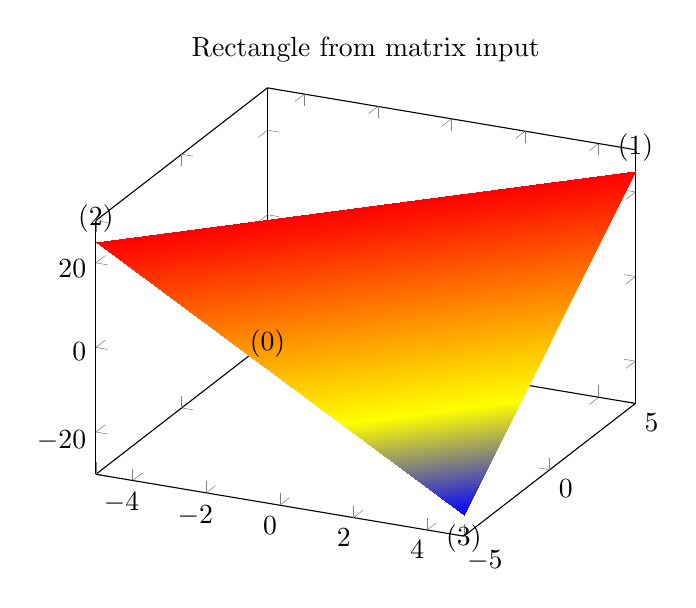
\begin{tikzpicture}
\begin{axis}[nodes near coords={(\coordindex)},
	title=Rectangle from matrix input]
% note that surf implies 'patch type=rectangle'
\addplot3[surf,shader=interp,samples=2,
	patch type=rectangle] 
	{x*y};
\end{axis}
\end{tikzpicture}
\end{codeexample}
\begin{codeexample}[]
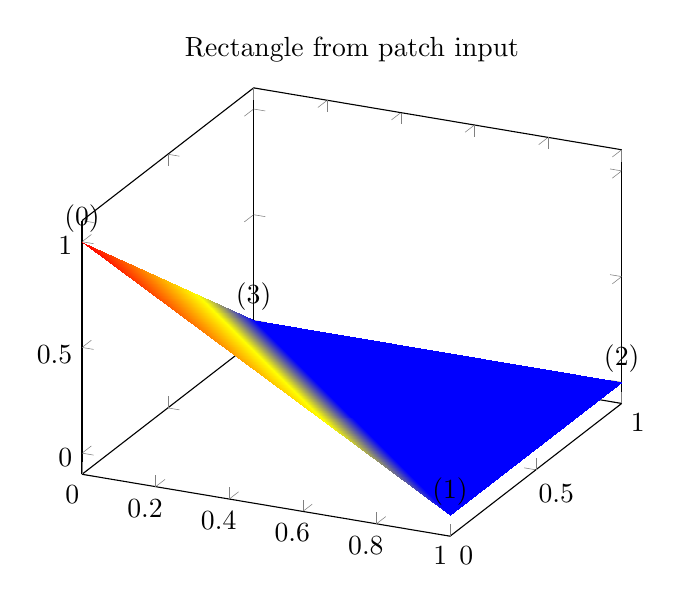
\begin{tikzpicture}
\begin{axis}[nodes near coords={(\coordindex)},
	title=Rectangle from patch input]
\addplot3[patch,shader=interp,patch type=rectangle] coordinates {
	(0,0,1) (1,0,0) (1,1,0) (0,1,0)
};
\end{axis}
\end{tikzpicture}
\end{codeexample}
	\noindent As already documented on page~\pageref{key:patch:type}, the |shader=interp| implementation for |rectangle| uses two triangles and interpolates them linearly. The differences between the two examples above arise due to $z$ buffering approaches: the matrix input reorders the matrix in linear time, whereas the second example would sort complete rectangles. In our case, this yields to the different corner sequence.

	The choice \declareandlabel{bilinear} is essentially the same as |rectangular| with respect to its input formats and stroke paths, but it uses correct bilinear shading for |shader=interp|. Moreover, the geometry is also interpolated bilinearly instead of just two triangles. The two examples from above now become
\begin{codeexample}[]
\begin{tikzpicture}
\begin{axis}[nodes near coords={(\coordindex)},
	title=Bilinear from $2\times 2$ matrix input]
% note that surf implies 'patch type=rectangle'
\addplot3[surf,shader=interp,samples=2,
	patch type=bilinear] 
	{x*y};
\end{axis}
\end{tikzpicture}
\end{codeexample}
\begin{codeexample}[]
\begin{tikzpicture}
\begin{axis}[nodes near coords={(\coordindex)},
	title=Bilinear from $4$--point patch input]
\addplot3[patch,shader=interp,patch type=bilinear] 
coordinates {
	(0,0,1) (1,0,0) (1,1,0) (0,1,0)
};
\end{axis}
\end{tikzpicture}
\end{codeexample}
	\noindent Use |patch type=bilinear| if you want to improve the shape of individual patches and the quality of the color interpolation. In contrast to the simpler |patch type=rectangle|, it might result in a huger output document.

	The choice \declaretext{triangle} expects a sequence of linear triangles, each encoded using $n=3$ vertices:
\begin{codeexample}[]
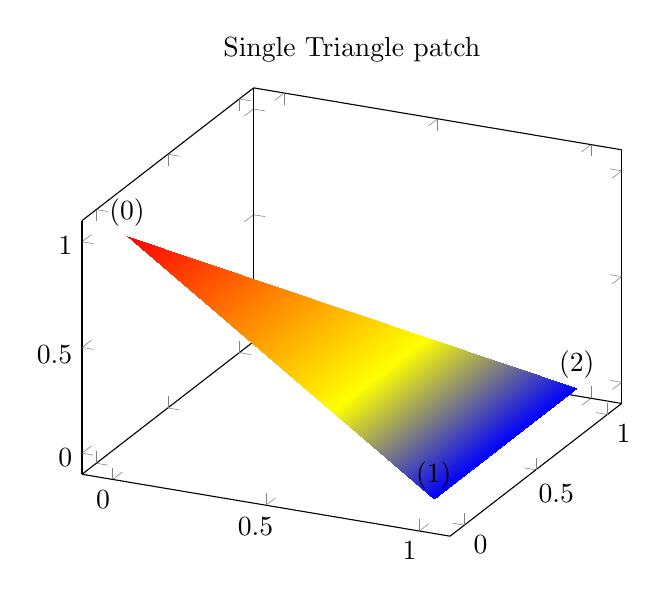
\begin{tikzpicture}
\begin{axis}[enlargelimits,
	nodes near coords={(\coordindex)},
	title=Single Triangle patch]
\addplot3[patch,shader=interp] coordinates {
	(0,0,1)
	(1,0,0)
	(1,1,0)
};
\end{axis}
\end{tikzpicture}
\end{codeexample}

	The choice \declareandlabel{triangle quadr} expects a sequence of isoparametric quadratic triangles, each defined by $n=6$ vertices:
\begin{codeexample}[]
\begin{tikzpicture}
\begin{axis}[nodes near coords={(\coordindex)},
	title=Quadratic Triangle]
\addplot[patch,patch type=triangle quadr,
	shader=interp,point meta=explicit]
coordinates {
	(0,0) [1] (5,4) [2] (0,7) [3]
	(2,3) [1] (3,6) [2] (-1,4)  [3]
};
\end{axis}
\end{tikzpicture}
\end{codeexample}
\begin{codeexample}[]
\begin{tikzpicture}
\begin{axis}[nodes near coords={(\coordindex)},
	title=Quadratic Triangle]
\addplot3[patch,patch type=triangle quadr,
	shader=interp]
coordinates {
	(0,0,1) (5,4,0) (0,7,0)
	(2,3,0) (3,6,0) (-1,4,0)
};
\end{axis}
\end{tikzpicture}
\end{codeexample}
	\noindent Here, the edges have the correct quadratic shape. However, the color interpolation is just \emph{bilinear}; using the color values of the corners and ignoring the rest (consider using |patch refines| to improve the color interpolation). For three dimensions, \PGFPlots\ checks the depth of corners to determine foreground/background. For two dimensions, strongly distorted elements may fold over each other in unexpected ways. 

	The choice \declareandlabel{biquadratic} expects a sequence of isoparametric biquadratic quadrilaterals each defined by $n=9$ vertices. Their main use is to get ``rectangles'' with smooth boundaries: 
\begin{codeexample}[]
\begin{tikzpicture}
\begin{axis}[nodes near coords={(\coordindex)},
	title=Single Biquadratic Quadrilateral]
\addplot[patch,patch type=biquadratic,
	shader=interp,point meta=explicit]
coordinates {
	(0,0) [1] (6,1) [2] (5,5) [3] (-1,5) [4]
	(3,1) [1] (6,3) [2] (2,6) [3] (0,3) [4]
	(3,3.75) [4]
};
\end{axis}
\end{tikzpicture}
\end{codeexample}
\begin{codeexample}[]
\begin{tikzpicture}
\begin{axis}[nodes near coords={(\coordindex)},
	title=Single Biquadratic Quadrilateral]
\addplot3[patch,patch type=biquadratic,shader=interp]
coordinates {
	(0,0,1) (6,1,0) (5,5,0) (-1,5,0)
	(3,1,0) (6,3,0) (2,6,0) (0,3,0)
	(3,3.75,0)
};
\end{axis}
\end{tikzpicture}
\end{codeexample}
	\noindent Similar to |triangle quadr|, the edges have the correct quadratic shape -- but the color interpolation is just \emph{bilinear}; using the color values of the corners and ignoring the rest. Again, ensure that the mesh width so small enough in order to improve the quality of the color interpolation (see also |patch refines|).

	Note that a function of $(x,y)$ is biquadratic if it is quadratic w.r.t.~$x$ if  $y=\text{const}$ and also quadratic w.r.t.~$y$ if $x=\text{const}$ (note that this is not an ``if and only if''). For example, $f(x,y) = x^2-y^2$ is biquadratic. Consequently, we can represent a surface plot of $f$ with just one biquadratic patch -- only the color interpolation is just bilinear. We do so using |\addplot table[z expr=|\meta{expression}|]|:
\pgfplotsexpensiveexample
\begin{codeexample}[]
\begin{tikzpicture}
    \begin{axis}
    \addplot3[patch,patch refines=3,
		shader=faceted interp,
		patch type=biquadratic] 
    table[z expr=x^2-y^2]
    {
        x  y
        -2 -2
        2  -2
        2  2
        -2 2
        0  -2
        2  0
        0  2
        -2 0
        0  0
    };
    \end{axis}
\end{tikzpicture}
\end{codeexample}
	\noindent We see that the shape's boundary is reconstructed exactly using the |biquadratic| patch. In addition, |patch refines| improves the (first order) color interpolation. Details for |patch refines| are discussed in Section~\ref{sec:lib:patchplots:refinement} and details and limitations regarding superimposed grid lines are discussed in Section~\ref{sec:lib:patchplots:grids}.

	Note that |biquadratic| can easily be combined with |patch type sampling| in order to sample an arbitrary |surf|ace plot with smooth boundaries.

	A patch with type |biquadratic| and |shader=interp| has a bounding box which is determined from the input vertices. Due to the high order of the patch, parts of the patch can be outside of that bounding box. This holds for all advanced patch types.
	\index{Patch plots!Bounding Box}

	The choice \declareandlabel{bicubic} is similar to |biquadratic|: it allows to defines two--dimensional patches whose boundary is defined by four cubic polynomials. Consequently, it allows very smooth boundaries -- especially since the viewer constructs these boundaries at every zoom level. A |bicubic| patch is constructed from $16$ points which are arranged in a $4\times4$ matrix. Each consecutive $16$ points make up a single |bicubic| patch. The $17$th point starts the next |bicubic| patch (just as for any other |patch type|).
\begin{codeexample}[]
\begin{tikzpicture}
\begin{axis}[nodes near coords={(\coordindex)},
	title=Single Bicubic Quadrilateral]
\addplot3[patch,patch type=bicubic,shader=interp]
coordinates {
	(0,0,1) (1,0,0) (2,0,0) (3,0,0)
	(0,1,0) (1,1,0) (2,1,0) (3,1,0)
	(0,2,0) (1,2,0) (2,2,0) (3,2,0)
	(0,3,0) (1,3,0) (2,3,0) (3,3,0)
};
\end{axis}
\end{tikzpicture}
\end{codeexample}
	Just as for |biquadratic|, the color interpolation of |bicubic| is (just) bilinear, even though the geometry is of higher order. The color interpolation uses the |point meta| values determined at the four corners of each patch; all other values of |point meta| are ignored by the shader (although their values are used to compute |point meta min| and |point meta max|).
\begin{codeexample}[]
\begin{tikzpicture}
\begin{axis}[
	title=Two Bicubic Patches]
\addplot3[patch,patch type=bicubic,
	shader=interp,point meta=explicit]
coordinates {
	(0,0,1)[1] (1,0,0)[0] (2,0,0)[0] (3,0,0)[0]
	(0,1,0)[0] (1,1,0)[0] (2,1,0)[0] (3,1,0)[0]
	(0,2,0)[0] (1,2,0)[0] (2,2,0)[0] (3,2,0)[0]
	(0,3,0)[0] (1,3,0)[0] (2,3,0)[0] (3,3,0)[0]

	(3,0,0)[0] (4,0,0)[0] (5,0,0)[0] (6,0,0)[0.7]
	(3,1,0)[0] (4,1,.5)[1](5,1,0)[0] (6,1,0)[0]
	(3,2,0)[0] (4,2,0)[0] (5,2,0)[0] (6,2,0)[0]
	(3,3,0)[0] (4,3,0)[0] (5,3,0)[0] (6,3,0)[0.1]
};
\end{axis}
\end{tikzpicture}
\end{codeexample}
	The previous example uses two patches of type |bicubic|. Note that the color data (|point meta|) has been provided explicitly -- and its values are only used at the corners (the |[1]| value after the point |(4,1,.5)| is ignored). Color interpolation of |bicubic| patches uses only the color data at the patch's corners. The remaining color data values are ignored. Note that if you leave the default (which is |point meta=f(x)| instead of |point meta=explicit|), the second patch will be blue. This is because the four corner vertices of the second patch define the color shading -- and their $z$ value is~$0$.

	Note that |bicubic| can easily be combined with |patch type sampling| in order to sample an arbitrary |surf|ace plot with smooth boundaries.

	Just as described for |biquadratic|, a patch with type |bicubic| and |shader=interp| can have a bounding box which is slightly smaller than the region which is actually drawn (because the bounding box is computed from the input points).

	The choice \declareandlabel{coons} expects a sequence of one or more Coons patches, made up of $n=12$ points each. A Coons patch is delimited by four cubic B\'ezier curves, with the end points attached to each other -- and the $n$ points provide the required control points for these curves in a specific ordering which is illustrated in the following example:
\begin{codeexample}[]
\begin{tikzpicture}
\begin{axis}[nodes near coords={(\coordindex)},
	width=12cm,
	title=A Coons Patch]
\addplot[mark=*,patch,patch type=coons,
	shader=interp,point meta=explicit] 
coordinates {
	(0,0)   [0] % first corner
	(1,-1)  [0] % Bezier control point between (0) and (3)
	(4,0.7) [0] % Bezier control point between (0) and (3)
	%
	(3,2)   [1] % second corner
	(4,3.5) [1] % Bezier control point between (3) and (6)
	(7,2)   [1] % Bezier control point between (3) and (6)
	%
	(7,1)      [2] % third corner
	(6,0.6)    [2] % Bezier control point between (6) and (9)
	(4.5,-0.5) [2] % Bezier control point between (6) and (9)
	%
	(5,-2)   [3] % fourth corner
	(4,-2.5) [3] % Bezier control point between (9) and (0)
	(-1,-2)  [3] % Bezier control point between (9) and (0)
};
\end{axis}
\end{tikzpicture}
\end{codeexample}
	\noindent The four cubic B\'ezier curves are \emph{equivalent} to \texttt{curveto} paths of \pgfname, i.e.\ to a sequence of the form \parg{corner 1}|.. controls|\parg{control point A}| and |\parg{control point B}| .. |\parg{corner 2}. The interpolated shading is bilinear. More precisely, a bilinear shading in the unit cube $[0,1]^2$ is initialised which is then mapped into the Coons patch such that the corners match. The color interpolation uses only the color data of the four corners, color values of intermediate control points are ignored for the shading (although their value will be respected for the upper and lower limit of color data). In contrast to the finite element patches, a Coons patch is inherently two--dimensional. While you can still use three--dimensional coordinates, \PGFPlots\ will draw the shading as you provide it, without checking for the depth information (as it does for the other |patch type|s). In other words: depending on the current |view| angle, the shading might fold over itself in unexpected ways.

	Even for two dimensions, Coons patches may fold over themselves. To determine which part is foreground and which part is background, the following rule applies: the four corner points $(0)$, $(3)$, $(6)$, $(9)$ are associated to the unit cube points $(u,v) = (0,0)$, $(0,1)$, $(1,1)$ and $(1,0)$, respectively. The edge between corner $(3)$ and $(6)$ (i.e. the one with $v=1$) is foreground, the edge between $(1)$ and $(9)$ is background. Thus, large values of $v$ are drawn on top of small values of $v$. If $v$ is constant, large values of $u$ are drawn on top of small values of $u$. Thus, reordering the patch vertices (choosing a different first vertex and/or reversing the sequence) allows to get different foreground/background configurations\footnote{Internally, \PGFPlots\ employs such mechanisms to map the higher order isoparametric patch types to Coons patches, sorting according their corner's depth information.}.

	Note that |patch type sampling| is unavailable for |patch type=coons| because the control points are no point evaluation of the same function.

	The choice \declareandlabel{tensor bezier} is similar to |patch type=coons|: it allows to define a bezier patch. However, it allows more freedom: it has $16$ control points instead of the $12$ of a |coons| patch. The four additional control points are situated in the center of each patch. This |patch type| generates \texttt{.pdf} shadings of type~$7$ (whereas |coons| patches are shadings of type~$6$). It has been added for reasons of completeness, although it has not been tested properly. Please refer to the specification of the \texttt{.pdf} format for details\footnote{If someone is willing to test it and document it, feel free to email me!}. The choice |tensor bezier| is actually \emph{the same} as |patch type=bicubic| -- except that |bicubic| automatically respects the view depth (foreground/background) and is given in a different by means of function evaluations rather than control points.
	
	Note that |patch type sampling| is unavailable for |patch type=tensor bezier| because the control points are no point evaluation of the same function.

	The choice \declareandlabel{polygon} expects polygons with a fixed number of vertices. This |patch type| requires the number of vertices as argument:
	\begin{pgfplotskey}{vertex count=\meta{count}}
		The number of vertices to be used for |patch type=polygon|. The number can be arbitrary. All input patches are expected to have this many vertices -- but it is acceptable if a patch uses the same vertex multiple times. This means that |patch type=polygon| accepts polygons with different numbers of vertices, but you need to apply some sort of ``manual padding''.
		
		This parameter is (currently) mandatory.
	\end{pgfplotskey}
	A |patch| plot with |patch type=polygon| simply connects the $n$=|vertex count| vertices in their order of appearance and closes the resulting path:
\begin{codeexample}[]
\begin{tikzpicture}
	\begin{axis}[view/h=120,xlabel=$x$,ylabel=$y$]
	\addplot3[
		opacity=0.5,
		table/row sep=\\,
		patch,
		patch type=polygon,
		vertex count=5,
		patch table with point meta={%
			% pt1 pt2 pt3 pt4 pt5 cdata
			0 1 7 2 2 0\\
			1 6 5 5 5 1\\
			1 5 4 2 7 2\\
			2 4 3 3 3 3\\
	}]
	table {
		x y z\\
		0 2 0\\%0
		2 2 0\\%1
		0 1 3\\%2
		0 0 3\\%3
		1 0 3\\%4
		2 0 2\\%5
		2 0 0\\%6
		1 1 2\\%7
	};
% replicate the vertex list to show \coordindex:
\addplot3[only marks,nodes near coords=\coordindex]
table[row sep=\\] {
0 2 0\\ 2 2 0\\ 0 1 3\\ 0 0 3\\ 
1 0 3\\ 2 0 2\\ 2 0 0\\ 1 1 2\\
};
	\end{axis}
\end{tikzpicture}
\end{codeexample}
	\noindent The example above defines the |patch| by means of a connectivity table (|patch table with point meta|) and a vertex list (the normal input coordinates of the plot): there are~$8$ vertices and~$4$ polygons. Note that~$2$ of these polygons are triangles, one has $4$ corners and only of them actually has all~$5$ allocated corners. This effect can be achieved by replicating one of the corners. The connectivity table in our example defines a unique color for each polygon: $0$ for the first patch, $1$ for the second, $2$ for the third, and $3$ for the last. These numbers map into the current |colormap|.
	
	The |patch type=polygon| supports \emph{neither} triangulation \emph{nor} shading \emph{nor} refinement. The order of appearance of the input points is supposed to be the order in which the line--to operations of the resulting path are generated.




\subsection{Automatic Patch Refinement and Triangulation}
\label{sec:lib:patchplots:refinement}
\PGFPlots\ supports automatic patch refinement for most of its |patch type|s. There are mainly two purposes for patch refinement: to increase the quality of |z buffer=sort| and/or to improve color interpolation for high--order patches. 

\begin{pgfplotskey}{patch refines=\marg{levels} (initially 0)}
	This key controls patch refinement. The initial choice |patch refines=0| disables refinement and visualizes elements as they have been found in input files.

	A positive \meta{levels} enables (recursive) patch refinement: each patch is refined individually. 

	The following example illustrates the |patch refines| feature for a |triangle quadr| shape function on an edge. Note that since \PGFPlots\ uses only first order shading which is based on the corner points $(0)$, $(1)$ and $(2)$, the specified shape function of |patch refines=0| has constant color. Higher \meta{levels} approximate the patch with increasing quality:
\begin{codeexample}[]
\foreach \level in {0,1,2} {%
	\begin{tikzpicture}
	\begin{axis}[
		nodes near coords={(\coordindex)},
		footnotesize,
		title={patch refines=\level}]

	\addplot3[patch,patch type=triangle quadr,
		shader=faceted interp,patch refines=\level]
	coordinates {
		(0,0,0) (5,4,0) (0,7,0)
		(2,3,0) (3,6,1) (-1,4,0)
	};
	\end{axis}
	\end{tikzpicture}
}
\end{codeexample}
	\noindent In this example, patch refinement makes a huge difference since it is just one element with huge displacements. For practical examples, you probably won't need many refinement levels.
	
	The refined patches reproduce the geometry's shape exactly. In addition, they improve color interpolation. Note that its purpose is just visualization, therefor hanging nodes are allowed (and will be generated by |patch refine| for most |patch type|s).

	Patch refinement is implemented for all supported patches except for |patch type=coons|, |tensor bezier|, |bicubic| (might follow eventually) and |polygon|.
\end{pgfplotskey}

\begin{pgfplotskey}{patch to triangles=\mchoice{true,false} (initially false)}
	Occasionally, one has a complicated |patch type| on input and would like to visualize it as a |triangle| mesh. \PGFPlots\ supports automatic triangulation of patches. Triangulation means to replace each individual input patch by one or more triangles. Triangulation can be combined with |patch refines| in which case |patch refines| is applied first and the resulting refined patches are then triangulated.
\begin{codeexample}[]
\foreach \level in {0,1,2} {%
	\begin{tikzpicture}
	\begin{axis}[
		nodes near coords={(\coordindex)},
		footnotesize,
		title={Triangulation + \level\ refines}]

	\addplot3[patch,patch type=biquadratic,shader=faceted interp,
		patch to triangles,patch refines=\level]
	coordinates {
		(0,0,0) (6,1,0) (5,5,0) (-1,5,0)
		(3,1,0) (6,3,0) (2,6,0) (0,3,0)
		(3,3.75,1)
	};
	\end{axis}
	\end{tikzpicture}%
}
\end{codeexample}
	
	For one--dimensional |patch type|s like |quadratic spline|, |patch to triangles| results in approximation by means of |patch type=line| instead of |triangle|. 

	The |patch to triangles| feature is implemented for all supported patches except for |patch type=coons|, |tensor bezier|, and |polygon|.
\end{pgfplotskey}

\subsection{Peculiarities of Flat Shading and High Order Patches}
\label{sec:lib:patchplots:flat}
The |patchplots| library has been optimized for use with interpolated shadings, i.e.\ for |shader=interp|: it allows the filled area to fold over itself or to be outside of the patch boundaries.

\PGFPlots\ also supports |shader=flat| and |shader=faceted| by simply stroking and/or filling the patch boundaries. Naturally, such an approach works only if the enclosed patch boundary and the filled area are essentially the same! Consider using |shader=flat| or |shader=faceted| only if the \emph{mesh width is small enough} such that patches do not fold over themselves.

The following example illustrates the effect: the coarse single element on the left folds over itsself, resulting in strange fill patterns. Refining the mesh reduces the effect.
\begin{codeexample}[]
\foreach \level in {0,1,2} {%
	\begin{tikzpicture}
	\begin{axis}[
		footnotesize,
		title={Faceted + \level\ refines}]

	\addplot3[patch,patch type=biquadratic,shader=faceted,
		patch refines=\level]
	coordinates {
		(0,0,1) (6,1,0) (5,5,0) (-1,5,0)
		(3,1,0) (6,3,0) (2,6,0) (0,3,0)
		(3,3.75,0)
	};
	\end{axis}
	\end{tikzpicture}
}
\end{codeexample}

\subsection{Drawing Grids}
\label{sec:lib:patchplots:grids}
The |patchplots| library supports grid (|mesh|) visualization in the same way as for two/three--dimensional |mesh|- and |surf| plots. This includes four different approaches: the first is |shader=faceted|, which uses constant fill color and |faceted color| for stroke paths (as we already saw in Section~\ref{sec:lib:patchplots:flat}). The second approach is to use |shader=faceted interp| which uses interpolated shadings for filling and issues stroke paths on top of each interpolated element. The third approach is to issue two |\addplot| commands, one with the filled |patch| plot, and one with a |patch,mesh| style which only draws (colored) grid lines on top of the previous plot. The three approaches are shown below.
\begin{codeexample}[]
\begin{tikzpicture}
\begin{axis}[
	title={Grids with shader=faceted}]

\addplot3[patch,patch type=biquadratic,
	shader=faceted,patch refines=3]
coordinates {
	(0,0,1) (6,1,1.6) (5,5,1.3) (-1,5,0)
	(3,1,0) (6,3,0.4) (2,6,1.1) (0,3,0.9)
	(3,3.75,0.5)
};
\end{axis}
\end{tikzpicture}
\end{codeexample}
\noindent As already discussed in Section~\ref{sec:lib:patchplots:flat}, the approach with |shader=faceted| works well if the mesh width is small enough (such that single patches do not overlap and their fill area is within the patch boundaries).
%
\begin{codeexample}[]
\begin{tikzpicture}
\begin{axis}[
	title={Grids with shader=faceted interp}]

\addplot3[patch,patch type=biquadratic,
	shader=faceted interp,patch refines=3]
coordinates {
	(0,0,1) (6,1,1.6) (5,5,1.3) (-1,5,0)
	(3,1,0) (6,3,0.4) (2,6,1.1) (0,3,0.9)
	(3,3.75,0.5)
};
\end{axis}
\end{tikzpicture}
\end{codeexample}
\noindent Here, grid lines are defined to be the patch boundary, so it may occasionally happen for coarse patches that grid lines cross the filled area. If you experience problems, consider using the |patch refines| key. The |shader=faceted interp| supports |z buffer| -- at the cost of generating one shading for \emph{each} patch element (the stroke path is drawn immediately after the patch element is shaded). This can become quite expensive\footnote{I would really like to hear any well--founded ideas how to improve this issue. In case you have an idea-- let me know!} at display time and may lead to huge pdf files. However, |shader=faceted interp| provides smooth shadings and, at the same time, good  grid lines which are drawn in the correct order. 

%
\begin{codeexample}[]
\begin{tikzpicture}
\begin{axis}[
	title={Mesh on top of patches (i): obscured}]

\addplot3[patch,patch type=biquadratic,shader=interp,
	patch refines=3]
coordinates {
	(0,0,1) (6,1,1.6) (5,5,1.3) (-1,5,0)
	(3,1,0) (6,3,0.4) (2,6,1.1) (0,3,0.9)
	(3,3.75,0.5)
};
\addplot3[patch,patch type=biquadratic,mesh,black,
	patch refines=3]
coordinates {
	(0,0,1) (6,1,1.6) (5,5,1.3) (-1,5,0)
	(3,1,0) (6,3,0.4) (2,6,1.1) (0,3,0.9)
	(3,3.75,0.5)
};
\end{axis}
\end{tikzpicture}
\end{codeexample}
%
\begin{codeexample}[]
\begin{tikzpicture}
\begin{axis}[
	title={Mesh on top of patches (ii): unobscured\\
	  \tiny Geometry provided by Prof. Chernov, Bonn},
	title style={align=center},
	view={156}{28}]
\addplot3[patch,patch type=bilinear,
	shader=interp,
	patch table=plotdata/patchexample_conn.dat] 
	file {plotdata/patchexample_verts.dat};

\addplot3[patch,patch type=bilinear,
	mesh,black,
	patch table=plotdata/patchexample_conn.dat] 
	file {plotdata/patchexample_verts.dat};
\end{axis}
\end{tikzpicture}
\end{codeexample}
\noindent The approach to draw grids separately is done by means of two |\addplot| statements; the first using |patch| as before, the second using |patch,mesh|. This configures \PGFPlots\ to visualize just the mesh. Make sure you provide `|mesh|' after `|patch|' since the latter activates filled |surf| visualization. The approach of meshes on top of patches implies to draw grid lines simply over any previous drawing operations. Thus, depth information is lost (as displayed in the first example above). Overlaying grid lines on top of the surface works in special cases (see bottom picture). An approach which always works is to provide the mesh at a fixed $z$ position as displayed in the following example:
%
\begin{codeexample}[]
\begin{tikzpicture}
\begin{axis}[
	title={Separate Grids (iii)}]

\addplot3[patch,patch type=biquadratic,shader=interp,
	patch refines=3]
coordinates {
	(0,0,1) (6,1,1.6) (5,5,1.3) (-1,5,0)
	(3,1,0) (6,3,0.4) (2,6,1.1) (0,3,0.9)
	(3,3.75,0.5)
};
\addplot3[patch,patch type=biquadratic,
	mesh,black,
	z filter/.code={\def\pgfmathresult{1.8}},
	patch refines=3]
coordinates {
	(0,0,1) (6,1,1.6) (5,5,1.3) (-1,5,0)
	(3,1,0) (6,3,0.4) (2,6,1.1) (0,3,0.9)
	(3,3.75,0.5)
};
\end{axis}
\end{tikzpicture}
\end{codeexample}
\noindent Here, the first |\addplot3| command is the same as above, just with |shader=interp|. The second reproduces the same geometry, but uses a |z filter| to fix the $z$ coordinate (in this case to $z=1.8$). This effectively overrules all $z$ coordinates.

	Thus, grid lines can be drawn either by means of flat fill color with |shader=faceted| (efficient), by means of interpolated fill colors with |shader=faceted interp| (inefficient, see above) or, for special applications, using a separate |patch,mesh| plot which is drawn on top of the patches (efficient). In any case, the mesh visualization considers the |faceted color| which can depend on |mapped color|.

\end{pgfplotslibrary}
}
